\chapter{Introduction}

The purpose of this report is to provide a general and pedagogical higher level understanding of SuperBIT. The report structure is as follows; I begin by providing an overview of the instrument and how it operates. I then present the the reader with the theoretical background necessary to understand the forecasted data analysis process as well as appreciate the challenges SuperBIT needs to overcome. Finally, I summaries some of my personal contributions to the instrument in the context of the upcoming September 2019 flight. 
  

\section{Astronomy From the Stratosphere}
Collecting astronomical data from the stratosphere via a balloon borne instrument presents a plethora of advantages many of which are unique to ballooning. As seen in \autoref{fig:atmos} an optical telescope operating in the stratosphere can observe radiation more efficiently than ground based observatories, this is especially true in the blue and near UV frequency range. Additionally, such an instrument would operate above significant atmospheric turbulence and can thus provide diffraction-limited resolutions. While a space based telescope can similarly address the shortcomings of ground based observations, launching a propellent-based vehicle is 100-1000 times more expensive. Given the relative low cost of ballooning and the short development timescale of balloon borne instruments, ballooning uniquely provides the opportunity of an iterative development process relying on multiple test flights to ensure smooth scientific operation. The instrument of interest in this report namely, SuperBIT is a balloon borne imaging telescope designed to utilize the advantages listed above.

\begin{figure}
    \begin{small}
        \begin{center}
            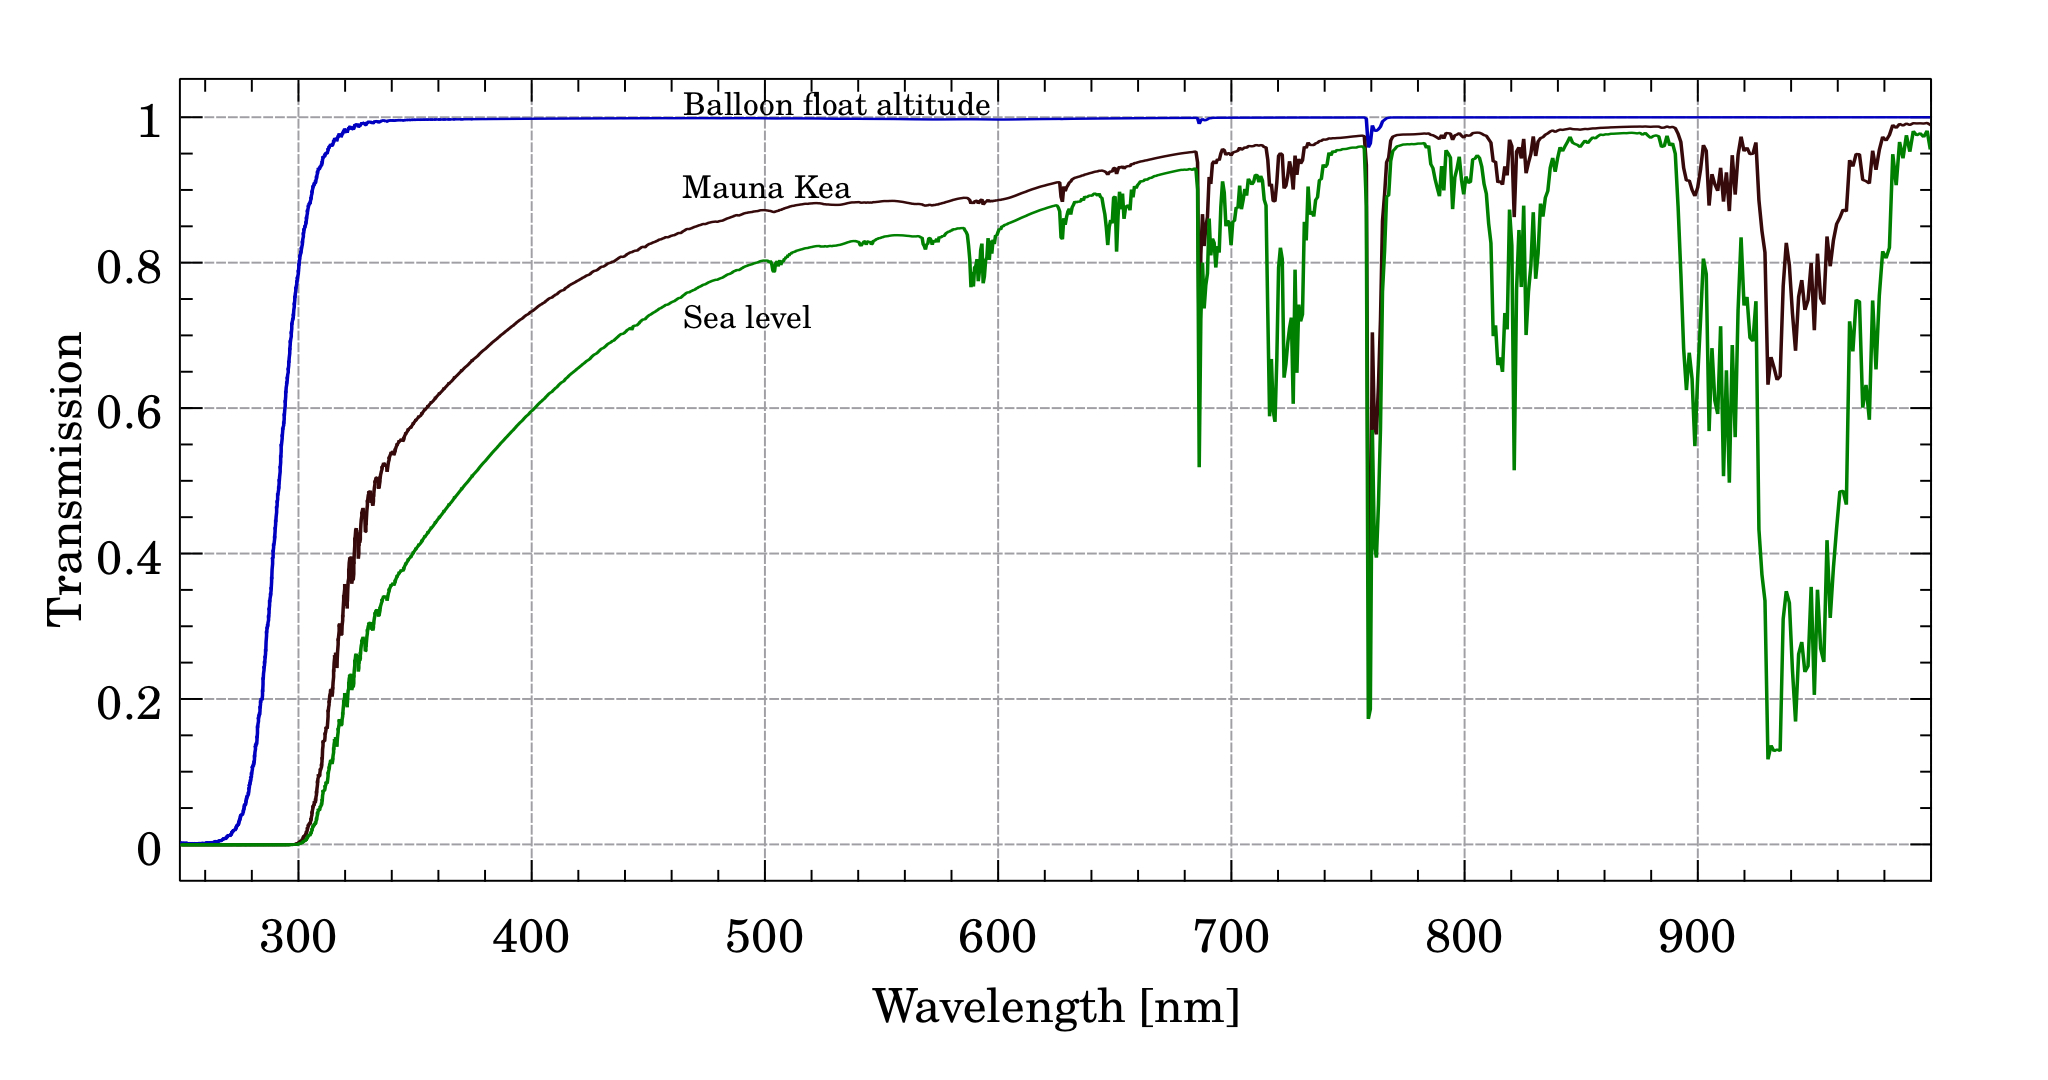
\includegraphics[width=0.95\textwidth]{Introduction/figs/atmosphere.jpg}
        \end{center}
        \caption{Transmission of the atmosphere vs wavelength at sea level (green), Mauna Kea (brown), and balloon float altitude (blue). It is clear that a balloon borne optical telescope provides a significant increase in exposure in the blue and near UV frequency range.}
        \label{fig:atmos}
    \end{small}
\end{figure}


\section{Super-pressure Balloon-borne Imaging Telescope (SuperBIT)}
SuperBIT is an optical to near UV balloon borne telescope providing diffraction-limited 0.25 arcsecond resolution imaging over a 0.4 degree filed of view with sensitivities exceeding 24th magnitude in 300 seconds of integration. SuperBIT is designed for an ultra-long duration balloon (ULDB) 100 day flight with the immediate science goal of providing precision weak and strong lensing mass measurements for more than 150 clusters.

\begin{figure}
    \begin{small}
        \begin{center}
            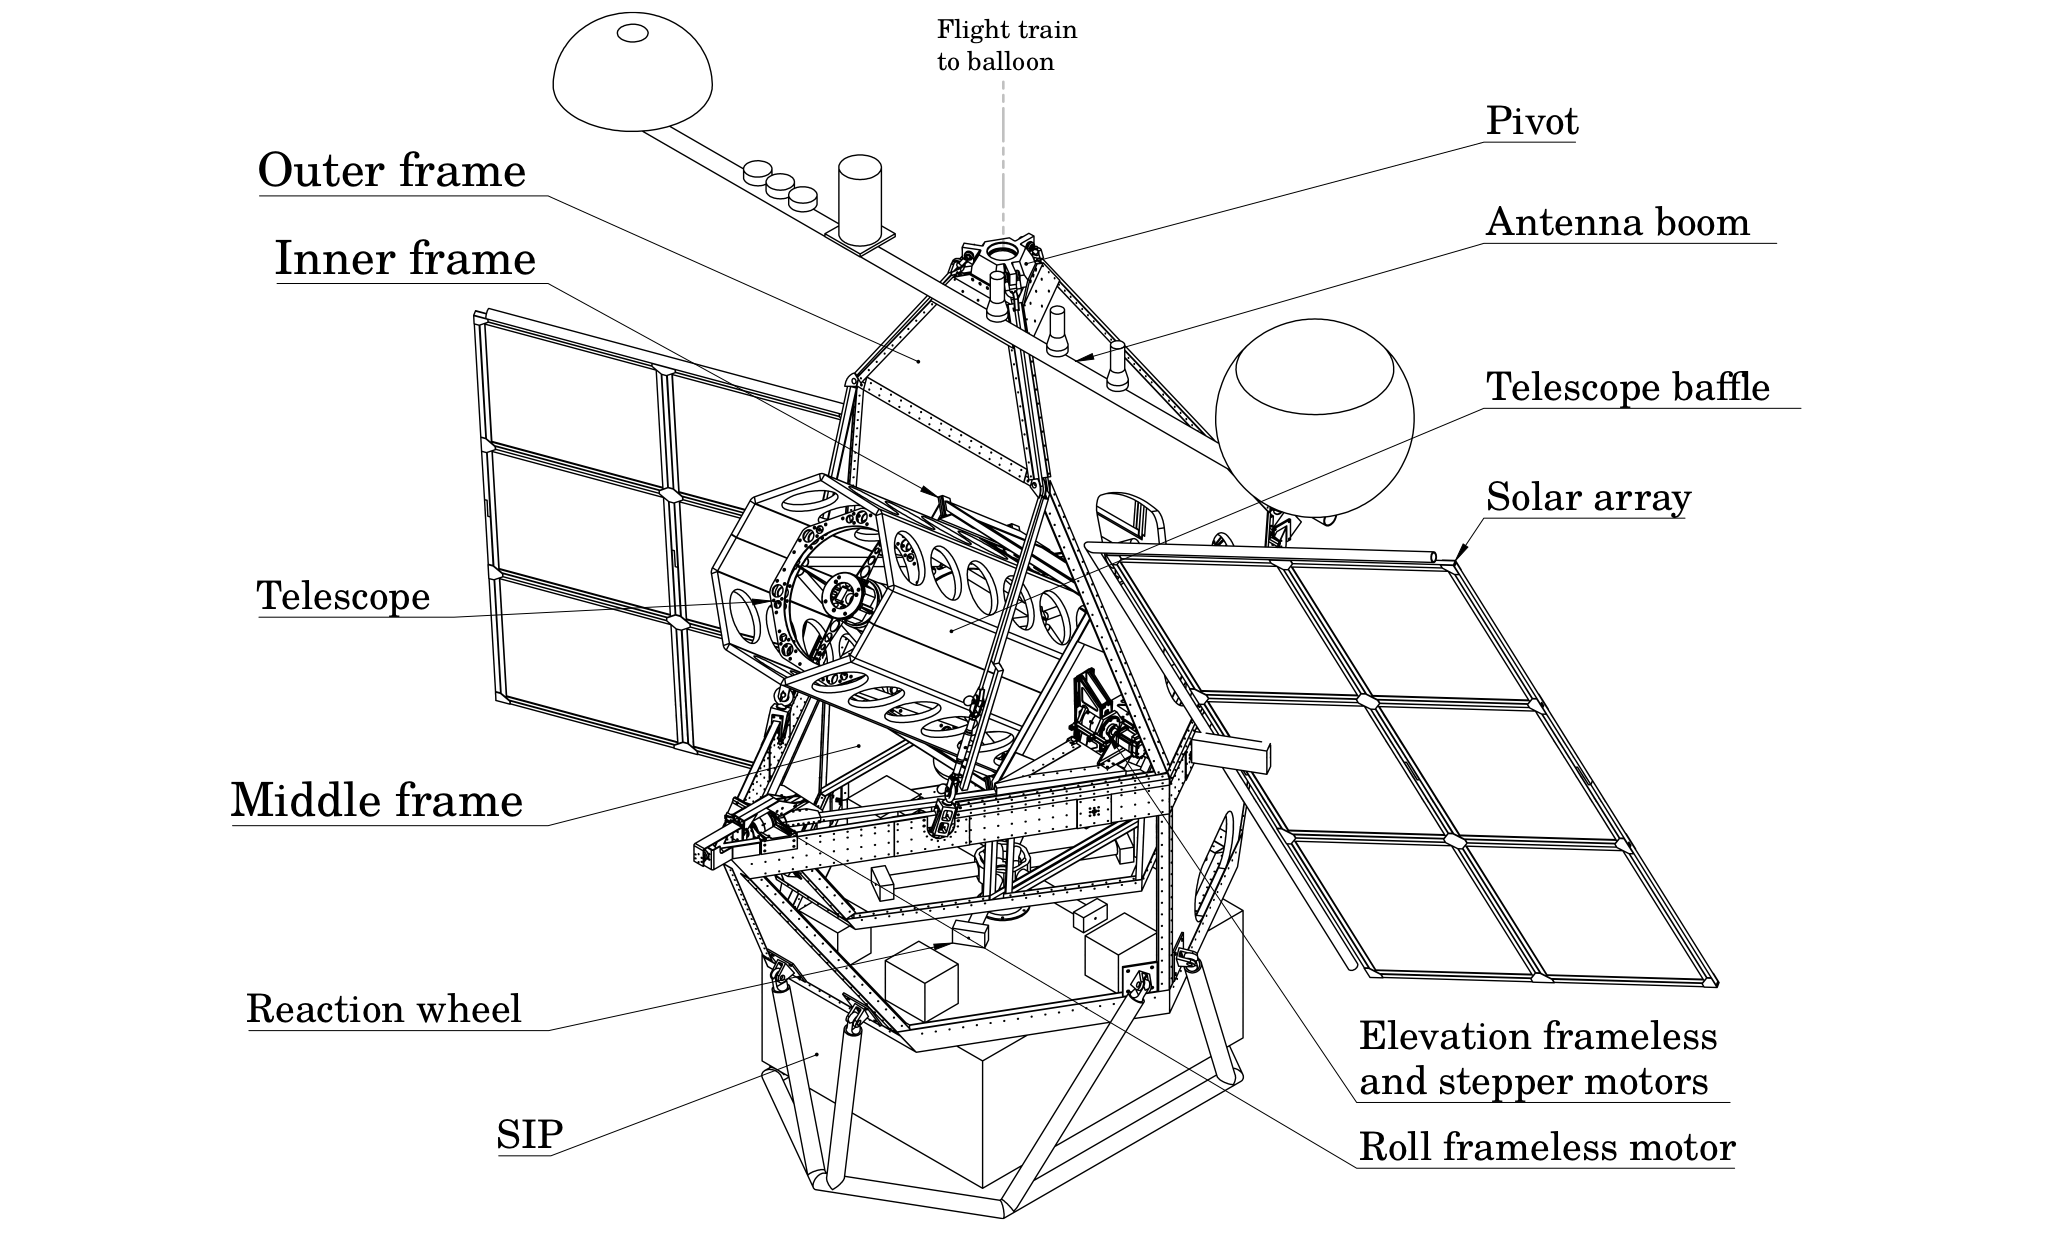
\includegraphics[width=0.95\textwidth]{Introduction/figs/bit_model.png}
        \end{center}
        \caption{Layout of the SuperBIT instrument.}
        \label{fig:bit}
    \end{small}
\end{figure}

\begin{figure}
    \begin{small}
        \begin{center}
            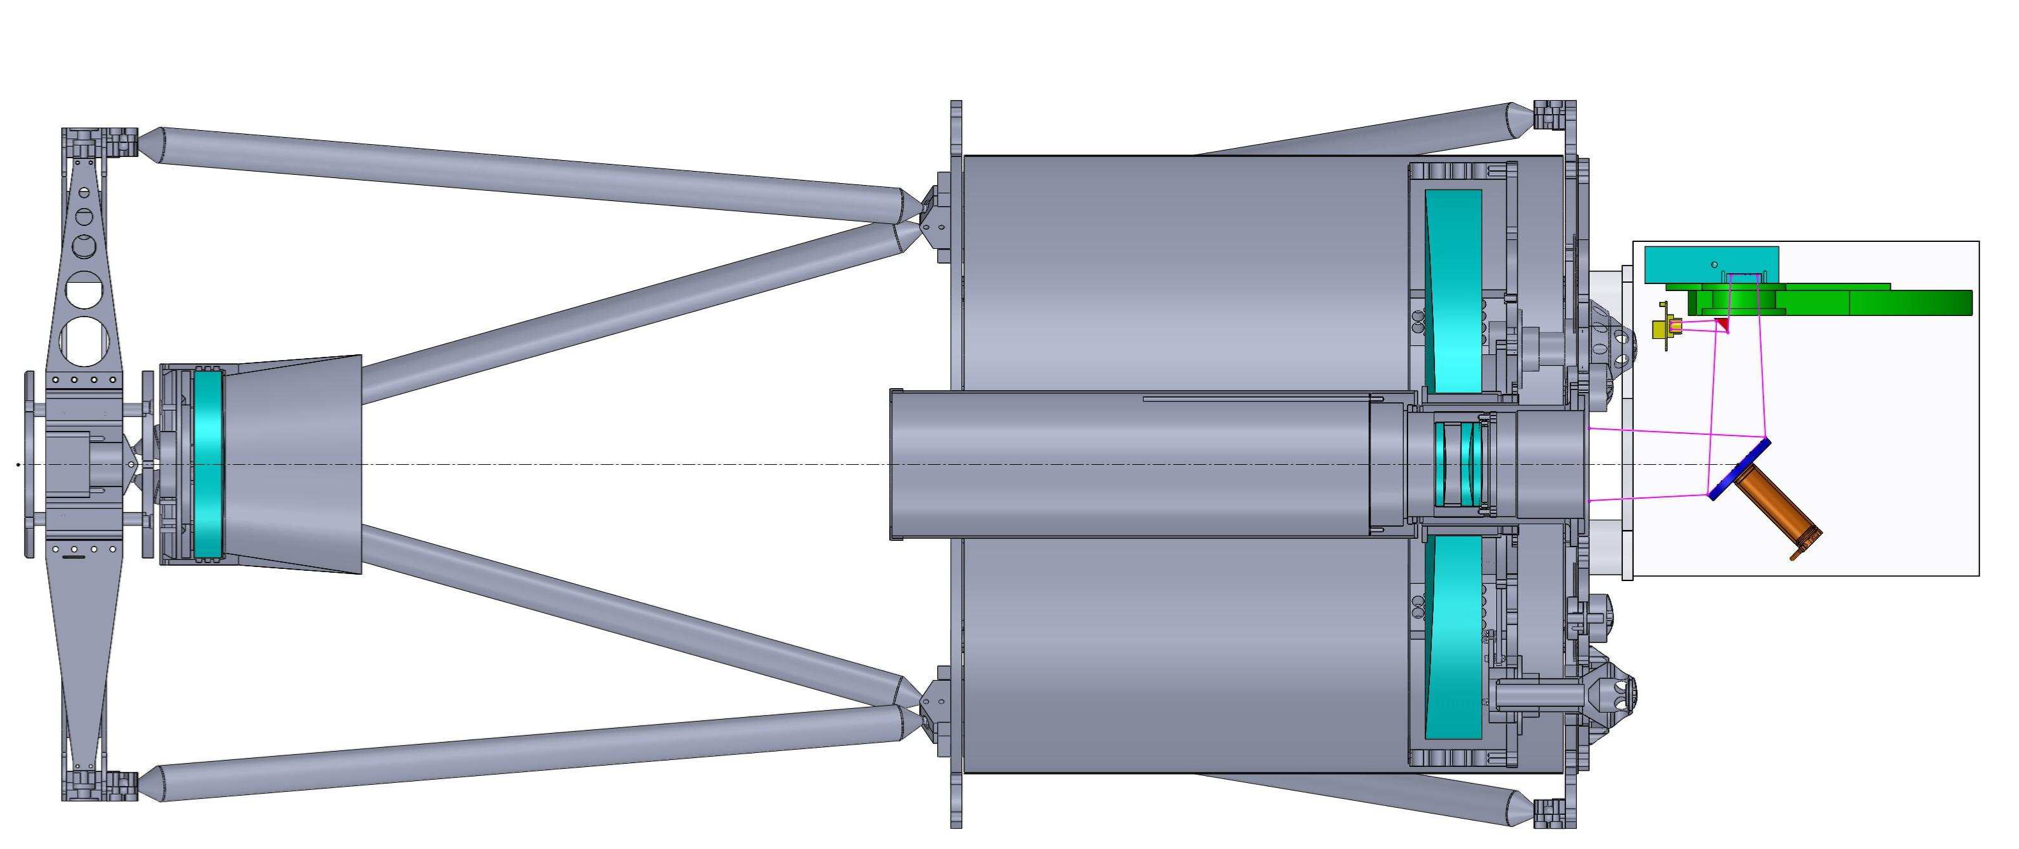
\includegraphics[width=0.95\textwidth]{Introduction/figs/optical_path.png}
        \end{center}
        \caption{The optical layout; The optical path (violet lines) is fed into the fine guidance system through the telescope (grey). The Tip/Tilt mirror (gold and blue) redirects the optical axis 90 degrees to the Science camera (cyan) through a filter wheel (green). Just before the filter wheel some of the light is redirected again by the pick-off mirror (red) to a star camera (yellow).}
        \label{fig:optics}
    \end{small}
\end{figure}

\par
For a more detailed description of the instrument please consult group alumni theses. For details on the electrical distribution systems and
superBIT mechatronics please see John Hartley's PhD thesis, for the mechanical structure see Steven Li’s Engineering Masters Thesis, for a detailed discussion of the controls system and software see Javier Romualdez’s PhD Thesis, for a detailed look at the star cameras system see Matthew Galloway’s PhD Thesis, and for details of the thermal control system see Susan Redmond’s Engineering Masters Theses.

